\chapter{Veileder i bruk av rotårsaksanalyse innen informasjonssikkerhet}
\label{kap:veiledning-RCA}
Veilederen er skrevet slik at de kan bli benyttet uten bacheloroppgaven. Derfor vil noe av det som er gjennomgått i bacheloroppgaven bli gjentatt.

\section{Formål og bakgrunn}
Formålet med dette dokumentet er å gi leseren en veileder for anvendelse av rotårsaksanalyse. Veilederen beskriver anvendelse av rotårsaksanalyseverktøyene beskrevet i boken ``Root Cause Analysis: Simplified Tools and Techniques - second edition'' av Bjørn Andersen og Tom Fagerhaug \cite{RCA} i forhold til informasjonssikkerhet. Vi anbefaler denne boken som samlet metodikk. Boken beskriver godt hva som skal til for å komme frem til rotårsaken til et problem. 

Dette dokumentet ble skrevet i forbindelse med bacheloroppgave i informasjonssikkerhet der det ble gjennomført tre caser. Veilederene er derfor basert på funn fra disse casene, om hvordan metoden og verktøyene fungerte.

Dette dokumentet vil ikke beskrive verktøyene, men valg av de. Beskrivelsen til verktøyene står i boken til Fagerhaug og Andersen \cite{RCA}.

\section{Valg av verktøy}
Boken beskriver 7 faser i rotårsaksanalyse. Disse må bli fulgt stegvis ettersom hver fase bygger på resultater fra foregående. Verktøyene beskrevet i boken til Fagerhaug og Andersen \cite{RCA} er generelle verktøy som er ofte brukt i rotårsaksanalyse. Vi har sett på et utvalg av disse verktøyene og hvordan disse fungerer innen informasjonssikkerhet. Figur \ref{fig:prosess_veileder} under viser verktøyene i metodikken, og er fargekodet ut i fra hva vi anbefaler. 

\begin{figure}[H]
    \centering
    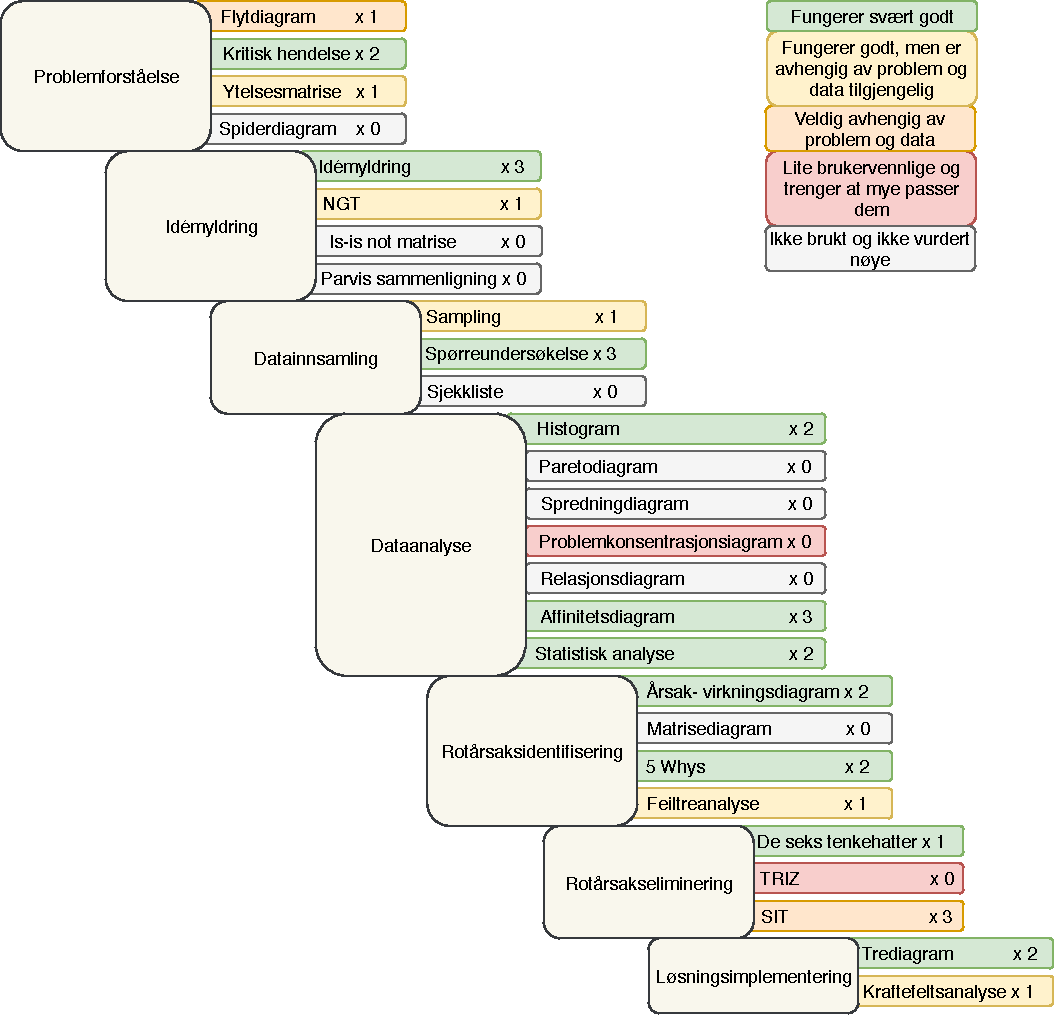
\includegraphics[scale=0.6]{main/bilder/RCA_Prosess_rettningslinjer.pdf}
    \caption[RCA-prosess]{De syv fasene i rotårsaksanalyseprosessen}
    \label{fig:prosess_veileder}
\end{figure}

\subsection{Problemforståelse}
Problemforståelse går ut på å få en solid forståelse for problemet en ønsker å løse. Det kan også hjelpe med å skape enighet i teamet rundt hva problemet egentlig omfatter. Det er også viktig for å passe på at ressursene som benyttes for analysen brukes effektivt videre. 
Verktøyene vi anbefaler til denne fasen er: 

\subsubsection{Kritiske hendelser} 
Kritiske hendelser er et godt verktøy å bruke når man har mye data som kan gi et innblikk i hva som går galt. Etter vår erfaring kan man bruke logger til å finne de kritiske hendelsene, hvilket passer utmerket i et informasjonssikkerhetsperspektiv. For kritiske hendelser i informasjonssikkerhet anbefaler vi at det utføres slik: 
\begin{description}
    \item [Steg 1: Logg tilgjengelig] Bruk informasjon fra hendelseslogger til å finne informasjon om kritiske hendelser.
    \item [Steg 1: Informasjon ikke i logg] Om hendelsene ikke er logget, kan informasjon hentes fra personell som jobber med hendelsene, eller samles inn selv.
    \item [Steg 2:] Sorter hendelsene etter frekvens.
    \item [Steg 3:] Bruk de mest kritiske hendelsene som startpunkter for analysen.
\end{description}


\subsection{Idémyldring}
Målet med idémyldring er å generere så mange idéer som mulig om et gitt emne. I rotårsaksanalyse er målet stort sett å generere en liste over problemområder som kan forbedres, identifisere mulige konsekvenser, generere en liste over mulige årsaker til problemet og oppmuntre til å tenke på løsninger som kan eliminere problemet. Verktøyene vi anbefaler til denne fasen er:

\subsubsection{Idémyldring} Idémyldring gir mange idéer om mulige rotårsaker. Vi brukte idémyldring på våres tre caser og fant verktøyet til å fungere strålende. Skulle det være noen i gruppen som dominerer myldringen, anbefales heller idéskriving. Dette verktøyet fungerer på samme måte som idémyldring, men istedenfor å si idéene høyt, blir de skrevet ned og samlet inn før de skrives på tavlen. 

\begin{description}
    \item[Steg 1:] Skriv opp problemstillingen en ønsker å ta utgangspunkt i på en tavle og la personene i gruppen komme med idéer. Husk på å ikke kritisere idéene til hverandre. Prosessen burde la seg dø ut en gang for å sørge for at alle idéer er nevnt. 
    \item[Steg 2:] Sorter alle idéene i grupper og gå videre med de mest lovende idéene.
\end{description}

\subsubsection{Nominell gruppe teknikk} 
Dette verktøyet gir en liste over hva en burde prioritere mest i datainnsamling for å gi ett mer målrettet datagrunnlag for å finne rotårsaken. Vi anbefaler å bruke dette verktøy som et supplement, skulle man ha mange idéer fra idémyldringen og trenger å prioritere.
\begin{description}
    \item[Steg 1:] Gi hver idé fra idémyldringen hver sin bokstav.
    \item[Steg 2:] Gi alle gruppemedlemene hvert sitt stemmeark, med alle bokstavene på. 
    \item[Steg 3:] Gi fem idéer et tallpoeng fra 1-5 der 5 selvfølgelig er høyest.
    \item[Steg 4:] Tell opp poengsummene. De idéene med flest poeng prioriteres videre i prosessen.
\end{description}


\subsection{Datainnsamling}
Datainnsamling er et steg i prosessen der man skal være strukturert og samle inn så mye relevant informasjon om problemstillingen som mulig. En god datainnsamling er sentralt for gode resultater i senere faser. Vi anbefaler følgende verktøy:

\begin{description}
    \item[Sampling] Sampling er et godt verktøy for å begrense datainnsamling til en utvalgt del av en større gruppe. Brukes ofte i kombinasjon ble spørreundersøkelser eller sjekklister.
    \item[Spørreundersøkelser] Spørreundersøkelser er et godt verktøy for å få data fra de berørte personene.
\end{description}

\subsection{Dataanalyse}
I denne fasen blir dataene analysert og visualisert. Hovedmålet er å avklare mulige rotårsaker som har innvirkning på problemet, og hvilke av de som har størst innflytelse. Under beskrives de ulike verktøyene som ble brukt for å analysere dataene. Verktøyene vi anbefaler til denne fasen er:
Når det gjelder histogram og statisk analyse vil vi ikke skrive noe om stegene som må tas, da det kommer an på hva programvare som brukes.

\begin{description}
    \item[Histogram] Histogram fungerer veldig godt for å skape en visuell forståelse av dataene, som kan gjøre det lettere å se korrelasjoner mellom variabler. Det gir også en tilfredstillende fremstilling av dataen. 
\end{description}

\subsubsection{Statistisk analyse}
Statistisk analyse er ikke i boken, men er en analyse metode som fungerer veldig godt for å se korrelasjoner. Dette fungerer også ved å se på signifikansen.
\begin{description}
    \item[Steg 1:] Alle svar til nummeric form
    \item[Steg 2:] Gjennomfør korrelasjon på svarene
    \item[Steg 3:] De som korrelerer, gjennomfør en One-Way ANOVA eller en uavhengig t-test avhengig om det er 2 eller flere grupper.
    \item[Steg 4:] Gjennomfør Histogram på de som har signifikans for å visualisere korelasjonen.
\end{description}

\subsubsection{Affinitetsdiagram} Affinitetsdiagram passer veldig godt med spørreundersøkelser, der det er kortsvar- eller langsvaroppgaver. Den gir mulighet for å gruppere svarene etter innhold i svarene. 
\begin{description}
    \item[Steg 1:] Bruk data fra forrige fase til å komme fram til mulige årsaker.
    \item[Steg 2:] Skriv årsakene på post-it lapp.
    \item[Steg 3:] Grupper årsakene. Ofte må årsakene flyttes flere ganger før gruppene blir funnet. Bør ikke overstige 5-10 grupper 
    \item[Steg 4:] Lag tittel på gruppene
\end{description}

\subsection{Rotårsaksidentifisering}
De foregående fasene skal ha generert en liste over mulige rotårsaker og målet i denne fasen er å identifisere de faktiske årsakene. 

Verktøyene vi anbefaler til denne fasen er:

    \subsubsection{Årsak-virkning diagram} Som årsak-virkning anbefaler vi å benytte fiskebeindiagram. Ved å bruke fiskebeindiagram får en en visuell fremstilling av rotårsaken til problemet.
    \begin{description}
        \item[Steg 1:] Tydelig definer hva problemstilingen er.
        \item[Steg 2:] Bruke Draw.io eller et annet tegneprogram til tegne fiskebeindiagramet.
        \item[Steg 3:] Identifisert hovedårsakene for problemstilingen og tegn de opp som greiner.
        \item[Steg 4:] Idémyldre alle årsak som kan knyttes til hovedårsakene.
        \item[Steg 5:] analyser årsak for å identifisere det som mest sannsynlig er rotårsaken
    \end{description}
    
\subsubsection{5 Whys} Hvis det er mistanke om høyere årsaker bak de identifiserte årsakene kan 5 whys gi en bekreftelse på om årsakene identifisert er faktisk rotårsak og ikke lav-nivå årsaker. Det kan kreve flere iterasjoner for å finne rotårsaken(e).  
    
\subsubsection{Feiltreanalyse} Brukes etter en 5 whys, for å få en visuell presentasjon på hvordan de forskjellige rotårsakene man kom frem til i 5 whys henger sammen.


\subsection{Rotårsakseliminering}
Denne fasen innebærer å komme med mulige løsninger til problemet for å eliminere rotårsaken. Boken til Fagerhaug og Andersen \cite{RCA} beskriver to mulige tilnærminger til denne fasen. En tilnærming for å stimulere kreativitet når man leter etter løsninger, og en for å konstruere og utvikle løsninger. Vi vil i denne fasen primært anbefale å bruke de seks tenkehatter med de modifikasjonene vi har gjort istedenfor å bruke SIT.

Verktøyene vi anbefaler til denne fasen er:
\subsubsection{De seks tenkehatter} Seks tenkehatter fungerer godt for å idéemyldre løsninger når all dataen er klar. Seks tenkehatter er også den måten vi tror passer best for rotårsakselimineringen.
    \begin{description}
        \item[Steg 1:] I seks tenkehatter er det 6 forskjellige fargede hatter som skal brukes i prosessen:
            \begin{description}
                \item[Hvit hatt] skal være kald, nøytral og objektiv, personen skal fokusere på fakta.
                \item[Rød hatt] skal representere sinne, og skal bare fokusere på magefølelsen og egne følelser.
                \item[Svart hatt] skal være pessimistisk og negativ, og fokusere på hvorfor idéen er dårlig.
                \item[Gul hatt] er optimistisk og positiv, og skal fokusere på hvorfor idéen er bra og vil fungere.
                \item[Grønn hatt] representerer gresset, fruktbarhet og vekst, og skal fokusere på å vøre kreativ og komme på nye idéer.
                \item[Blå hatt] er koblet til himmelen, og skal fokusere på å se tingene fra et høyere perspektiv.
            \end{description}
        \item[Steg 2:] Diskusjonen om problemet foregår hvor hver deltager tar utgangspunkt i hatten deres.
        \item[Steg 3:] Når alle idéene er ferdige går man videre med å bearbeide de mest lovende idéene, og videreutvikle disse.
    \end{description}
    
\subsubsection{SIT} Vi prøvde SIT i hver av casene våres for å se hvordan det fungerte. Vi kom fram til at SIT er et tungvint verktøy å starte, der bruk av SIT-prinsippene ikke godt lar seg overføre til informasjonssikkerhet. Resten av stegene går bra og gir gode resultater i form av forslag på en tiltaksplan.  
    \begin{description}
        \item[Steg 1:] Ideelt sett bør man bruk et team som består av personer som innehaver all mulig informasjon om problemet. Er mulig uten, men blir langt vanskeligere å gjøre.
        \item[Steg 2:] List alle komponenten og sørg for å ta med de som virker irrelevant. 
        \item[Steg 3:] Bruke de fem SIT-prinsippene:
                    \begin{description}
                    \item[Attributtavhengighet] vurderer å endre en nøkkelvariabel i et produkt for å skape forbedring.
                    \item[Komponentkontroll] ser på hvordan et produkt er knyttet til omgivelsene.
                    \item[Erstatning] handler om å erstatte en del av et produkt med noe annet fra produktets omgivelser.
                    \item[Forkastning] vurderer å forbedre problemet ved å fjerne en komponent. 
                    \item[Oppdeling] har som mål å splitte et produkts attributter i to, som for eksempel splittelsen av sjampo fra balsam.
                    \end{description}
        \item[Steg 4:] Velg de idé som er best egnet for videre utdyping
        \item[Steg 5:] Forsett med utdype idé og kom opp med en eller flere løsninger med en tiltaksplan.
    \end{description}

\subsection{Løsningsimplementering}
I den siste fasen er målet å implementere løsningene som ble funnet i foregående fase. Implementeringen inkluderer blant annet organisering, utvikling av en implementeringsplan, skape et konsensus om de nødvendige endringene og selvfølgelig implementeringen. Implementeringen av løsningen kan sies å være en suksess når symptomene forsvinner. 

Verktøyene vi anbefaler til denne fasen er:

\subsubsection{Trediagram} Trediagram fungerer veldig bra for å lage en plan over hva som må gjøres for at tiltaket skal bli implementert. 
\begin{description}
    \item[Steg 1:] Lag en liste over gjøremål for å implementere løsningen(e)
    \item[Steg 2:] Disse skal grupperes og settes opp i en trestruktur, i rekkefølgen som skal til for å få løsningen implementert.
\end{description}

I dette steget er det ikke nødvendig å bruke noe verktøy, men det kan være lurt å benytte trediagram for å få en plan over løsningimplementering.

